\section{Literature Review}

Fabric classification has been an area of growing interest in the fields of computer vision and material science due to its wide range of applications across industries such as fashion, healthcare, manufacturing, and forensics. With the advancement of deep learning, researchers have been exploring automated methods to accurately identify and classify textile materials using image data.

Traditionally, fabric classification relied on manual techniques and physical testing, but these approaches are time-consuming, prone to human error, and often require specialized equipment. In contrast, image-based classification using deep learning models offers a scalable and efficient alternative that can be used even in real-time applications.

In this section, we review key research contributions that have applied deep learning techniques for fabric classification. The datasets described here, used in these studies are carefully considered, as data quality and diversity are vital to achieving strong model performance. We also provide a detailed discussion of the three papers that were selected and implemented as part of this research work. Each paper highlights a different modeling approach offering valuable insights into the strengths and limitations of current methodologies.

By analyzing these works, we aim to identify the common practices, innovative ideas, and existing challenges in the domain, which in turn have shaped the direction of our proposed methodology.

\subsection{Dataset Overview}

The development of accurate and generalizable deep learning models for fabric classification is heavily dependent on the availability of high-quality, diverse, and well-structured datasets. Each dataset used in this domain captures textile properties from a unique perspective—some focus on fine surface-level textures, others provide microscopic or structural imaging, and some present large-scale image collections labeled through expert-driven taxonomies.

In this section, we present a detailed review of three key datasets that were used in the implementation and evaluation of deep learning models for this research. These datasets have been selected for their relevance, diversity, and their ability to represent different challenges in fabric classification. Each dataset has contributed to our understanding of how fabrics can be categorized based on visual cues, micro-structures, and material properties. The datasets reviewed are described below:

\subsubsection{A. Fine-Grained Material Classification Using Micro-geometry and Reflectance~\cite{kampouris2016fine}}

One of the foundational datasets used for fine-grained material classification is based on micro-geometry and reflectance properties. This dataset, introduced by Kampouris et al., captures subtle material differences through high-resolution images that include shape, surface detail, and reflectance captured under varying lighting conditions.

The dataset was developed to aid in distinguishing materials that are visually similar to the human eye but differ in their physical or optical properties. It includes a range of fabrics and other material surfaces, photographed under controlled settings using a multi-light camera rig. Each sample is captured from multiple angles and under multiple lighting directions to collect reflectance fields. This setup allows for capturing texture, gloss, and geometric cues that are often difficult to extract from standard RGB images.

\begin{figure}[H]
    \centering
    \begin{minipage}{0.8\linewidth}
        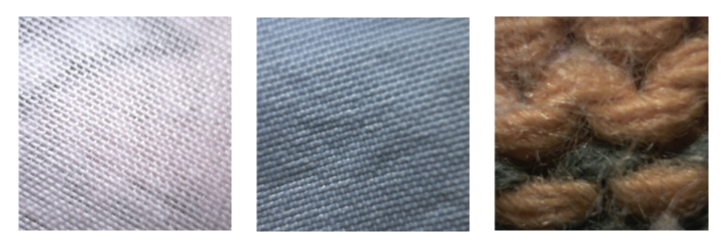
\includegraphics[width=\linewidth]{images/iBugDataset}
    \end{minipage}
    \caption[Sample images from the iBug Fabric Dataset]{Sample images from the iBug Fabric Dataset: (Left) Cotton, (Middle) Polyester, (Right) Wool.}
\end{figure}

What makes this dataset particularly useful for material classification is its emphasis on surface detail and reflectance behavior, rather than color or pattern alone. This makes it ideal for deep learning models that aim to identify materials based on physical characteristics, which are more consistent across environments compared to visual patterns.

Although the dataset covers a broader range of materials beyond textiles, its fabric subset is still highly valuable. It includes fabrics like cotton, wool, denim, and silk—each captured in fine detail—providing strong training data for distinguishing between these visually similar but structurally different materials.

This dataset serves as a strong foundation for deep learning models focused on material classification in fine-grained scenarios and is especially relevant when the goal is to distinguish fabrics based on their structural textures and reflectance rather than color or shape alone.

\subsubsection{B. Optical Coherence Tomography Image Dataset of Textile Fabrics~\cite{sabuncu2022optical}}

The Optical Coherence Tomography (OCT) image dataset of textile fabrics is a unique and specialized dataset that provides high-resolution cross-sectional images of fabric structures. Developed by Sabuncu and Ozdemir, this dataset aims to support material classification tasks through depth imaging and has proven useful for textile engineering, recycling, and forensic analysis.

The dataset includes OCT scans of fabrics made purely from cotton, wool, and polyester. For each material type, three different fabric samples were selected, resulting in a total of nine fabric categories. Using the Thorlabs CAL110C1 OCT system, each sample was scanned at over a hundred random surface locations to generate detailed cross-sectional images, commonly known as B-scans. The scan length was fixed at 2\,mm across all samples, and images were stored in raw \texttt{.png} format without any additional filtering or preprocessing.

\begin{figure}[H]
    \centering
    \begin{minipage}{0.8\linewidth}
        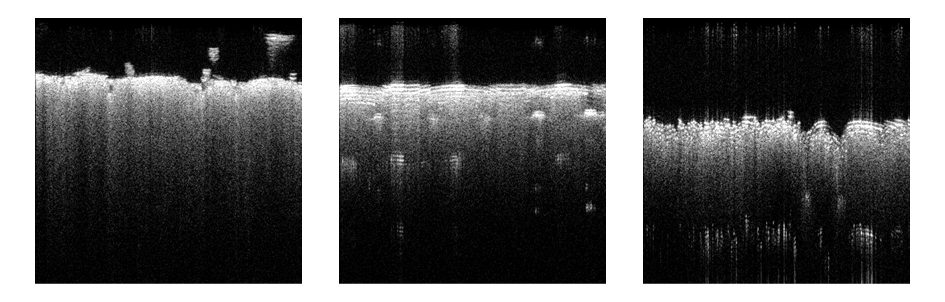
\includegraphics[width=\linewidth]{images/FabricOCTDataset.png}
    \end{minipage}
    \caption[Sample images from the Fabric OCT Dataset]{Sample images from the Fabric OCT Dataset: (Left) Cotton, (Middle) Polyester, (Right) Wool.}
\end{figure}

A key advantage of OCT imaging lies in its ability to reveal internal microstructural features of the fabric that are not visible in standard RGB images. These features include weave patterns, layer thickness, and material density, making OCT particularly valuable for classifying fabrics that may appear visually similar on the surface.

The dataset was structured into three main folders—cotton, wool, and polyester—each containing multiple scans from different fabric pieces of the same material. This setup provides a clean and well-labeled dataset that is suitable for training and testing deep learning models, especially those focused on learning from structural features rather than visual appearance alone.

Overall, the OCT image dataset offers a high degree of consistency and detail, which makes it ideal for tasks that require fine-grained classification of fabric types based on internal structure. Its application extends beyond classification, with potential uses in recycling processes, textile defect detection, and automated quality control in textile production.

\subsubsection{C. TextileNet: A Material Taxonomy-Based Fashion Textile Dataset~\cite{zhong2023textilenet}}

TextileNet is a large-scale, taxonomy-driven dataset designed to support textile material identification using deep learning techniques. Introduced by Shu Zhong et al., it addresses a major gap in existing datasets by providing a structured taxonomy of textile materials, divided into two primary categories: fibres and fabrics. Unlike most fashion-related datasets that often mix fibre and fabric labels or contain vague annotations, TextileNet provides a clearly defined and scientifically grounded label structure developed in collaboration with material science experts.

The dataset is split into two parts: \textit{TextileNet-fibre} and \textit{TextileNet-fabric}, comprising 33 fibre labels and 27 fabric labels, respectively. The total dataset consists of approximately 760,949 images, sourced from Google Images and reconstructed fashion datasets like iMaterialist. The image collection process was carefully curated using keyword-based queries derived from the defined textile taxonomies, ensuring that the dataset reflects real-world clothing items while maintaining a consistent label scheme.

\begin{figure}[H]
    \centering
    \begin{minipage}{0.8\linewidth}
        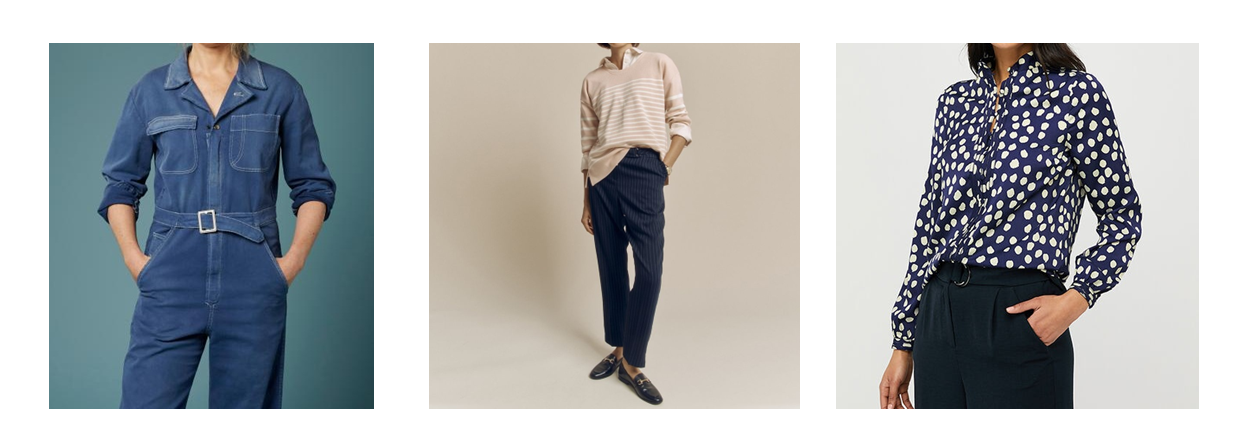
\includegraphics[width=\linewidth]{images/TextileNetDataset.png}
    \end{minipage}
    \caption[Sample images from the TextileNet Dataset]{Sample images from the TextileNet Dataset: (Left) Denim, (Middle) Crepe, (Right) Satin.}
\end{figure}

What makes TextileNet particularly valuable is its taxonomy-based design. The fibre taxonomy includes natural, synthetic, and regenerated fibres such as cotton, wool, polyester, bamboo viscose, and milk casein. The fabric taxonomy, on the other hand, categorizes textiles based on their production method (woven, knitted, non-woven) and includes examples like denim, tweed, velvet, and jersey.

% The dataset has been validated using both Convolutional Neural Networks (CNNs) and Vision Transformers (ViTs), with baseline models achieving over 80\% top-5 accuracy on classification tasks. It not only serves as a resource for textile classification but also supports sustainability-focused goals by enabling traceability of garments back to their fibre and fabric origins—a key step in promoting textile circularity.

Overall, TextileNet is suitable for training robust models that can identify complex fabric compositions in garments, supporting applications in retail, recycling, supply chain management, and sustainable fashion design.

\subsection{Existing Work}

In recent years, deep learning has shown remarkable progress in image-based classification tasks across various domains, including textiles. Numerous research efforts have applied Convolutional Neural Networks (CNNs) and Transformer-based architectures to classify fabrics and textile compositions with increasing accuracy and robustness. The integration of transfer learning and custom dataset preparation has further improved the performance of these models, even when working with limited or domain-specific data.

This section focuses on the review of selected research papers that have been implemented as part of this thesis. These papers represent different approaches to fabric classification—ranging from traditional CNN models to more advanced hybrid pipelines involving Vision Transformers and statistical techniques like Principal Component Analysis (PCA) and Linear Discriminant Analysis (LDA).

Each study has contributed significantly to the understanding of fabric classification challenges and techniques. By implementing and analyzing these works, we gain insights into the strengths and limitations of various deep learning models when applied to textile data. The outcomes from these implementations also provide the foundation for designing a more effective and efficient hybrid model tailored to the requirements of fine-grained fabric recognition.

\subsubsection[A. Research on Classification of Clothing Fabrics Images Based on Convolutional Neural Network]{A. Research on Classification of Clothing Fabrics Images Based on Convolutional Neural Network~\cite{hong2024research}}

In the paper \textit{“Research on Classification of Clothing Fabrics Images Based on Convolutional Neural Network”} by Ying Hong et al., the authors propose a deep learning-based approach to automatically classify clothing fabric types using image data. The main motivation behind the study is the growing need for intelligent fabric identification systems in clothing design and textile production, where manual classification can be time-consuming and inconsistent.

The authors utilize a transfer learning strategy by fine-tuning the VGG-16 model, a well-established convolutional neural network architecture, pre-trained on the ImageNet dataset. The study focuses on a custom dataset composed of 15,000 high-resolution images representing 10 different types of clothing fabrics, including cotton, wool, silk, denim, and others. The images are captured under controlled lighting conditions to ensure consistency and minimize background noise.

\begin{figure}[H]
    \centering
    \begin{minipage}{1\linewidth}
        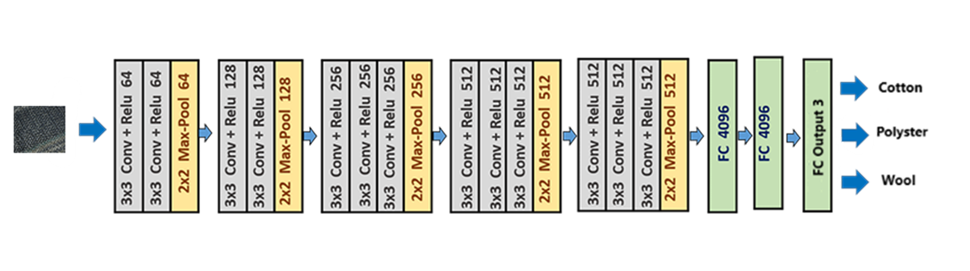
\includegraphics[width=\linewidth]{images/Paper1Model.png}
    \end{minipage}
    \caption[Model architecture - Hong et al.~\cite{hong2024research}]{Model architecture used for classification in Hong et al.~\cite{hong2024research}.}
\end{figure}

To enhance model generalization, the dataset undergoes data augmentation using techniques such as rotation, flipping, brightness adjustment, and the addition of Gaussian noise. These transformations help the network learn invariant features and reduce the risk of overfitting.

The proposed model achieves a test accuracy of 99.73\%, demonstrating high performance in distinguishing between visually similar fabric types. The authors also emphasize the model’s fast convergence rate and robust classification capabilities, suggesting that convolutional networks, even with moderate architectural depth like VGG-16, can be effectively employed for practical fabric recognition tasks.

This work highlights the advantages of combining transfer learning with carefully curated datasets and simple preprocessing steps. It confirms that CNN-based methods are well-suited for fabric classification, especially when high-quality image data is available. Additionally, the study provides a foundation for future research to explore more advanced architectures or multi-modal data sources, such as combining texture with reflectance or depth information.

\subsubsection[B. TextileNet: A Deep Learning Approach for Textile Fabric Material Identification from OCT and Macro Images]{B. TextileNet: A Deep Learning Approach for Textile Fabric Material Identification from OCT and Macro Images~\cite{siam2023textilenet}}

In the paper \textit{“TextileNet: A Deep Learning Approach for Textile Fabric Material Identification from OCT and Macro Images”} by Siam et al., the authors explore the use of deep learning models for automatic fabric material identification using two distinct types of images: macro images and Optical Coherence Tomography (OCT) scans. This work addresses the challenge of accurately classifying fabrics such as cotton, wool, and polyester, which often appear visually similar to the human eye but have distinct structural properties.

\begin{figure}[H]
    \centering
    \begin{minipage}{1\linewidth}
        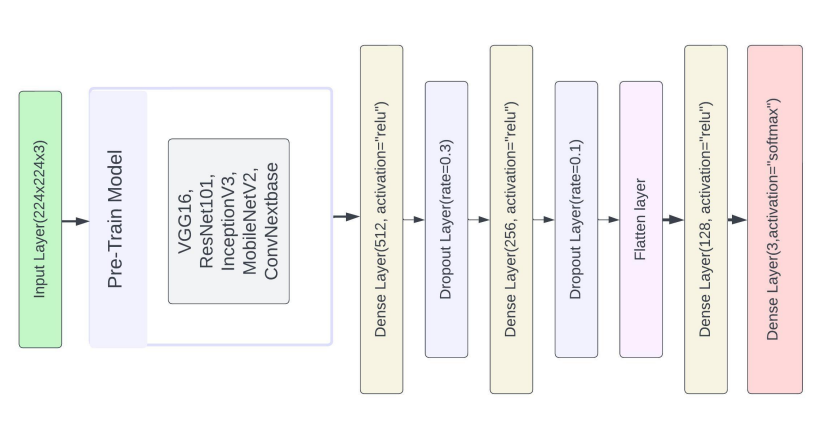
\includegraphics[width=\linewidth]{images/Paper2Model.png}
    \end{minipage}
    \caption[Model architecture - Siam et al.~\cite{siam2023textilenet}]{Model architecture used for fabric classification in Siam et al.~\cite{siam2023textilenet}}
\end{figure}

The study introduces a classification pipeline based on transfer learning, utilizing five pre-trained convolutional neural networks: MobileNetV2, VGG16, ResNet101, InceptionV3, and ConvNextBase. These models were adapted and fine-tuned to classify textile samples based on their visual and structural features.

To improve image quality and enhance model performance, preprocessing techniques such as grayscale conversion, contrast enhancement (CLAHE), and sharpening were applied. All images were resized to a standard input size of 224×224 pixels before being fed into the models.

The results demonstrate that MobileNetV2 outperformed the other models, achieving 99.87\% accuracy on OCT images and 95.17\% accuracy on macro images. The significant difference in performance between the two image types highlights the added value of using OCT imaging for fabric classification, as it reveals deeper structural features not visible in surface-level macro images.

This work shows that combining deep learning with high-resolution image modalities like OCT can lead to highly accurate and reliable fabric classification. The proposed pipeline is lightweight and efficient, making it suitable for real-world applications in the textile industry, such as automated material sorting, quality control, and textile recycling.

\subsubsection[C. Fabric Composition Identification using Fine-Tuned Vision Transformers]{C. Fabric Composition Identification using Fine-Tuned Vision Transformers~\cite{chitra2023fabric}}

The study \textit{“Fabric Composition Identification using Fine-Tuned Vision Transformers”} by Chitra G M et al. presents a modern approach to fabric classification by leveraging the capabilities of Vision Transformers (ViTs). Unlike traditional methods that rely solely on convolutional features, this work incorporates transformer-based architectures to extract and understand both local and global features in fabric images. The main goal of the study is to identify fabric compositions, especially in scenarios where fabrics may contain blends of multiple fibres.

The dataset used in the study consists of 937 images, each labeled with fabric compositions such as cotton, polyester, nylon, and silk. The images were captured using smartphone cameras, simulating a real-world setting where users or retailers may need to classify fabric types using accessible devices. This practical setup makes the proposed method more adaptable for mobile or on-site fabric recognition applications.

The proposed pipeline combines several stages. Initially, features are extracted from images using a fine-tuned ViT model. These features are then reduced using Principal Component Analysis (PCA) and further refined using Linear Discriminant Analysis (LDA) to enhance class separation. Finally, a Support Vector Machine (SVM) classifier is used for the final prediction. The authors also apply Platt scaling to calibrate the probability outputs of the SVM for better confidence estimation.

\begin{figure}[H]
    \centering
    \begin{minipage}{1\linewidth}
        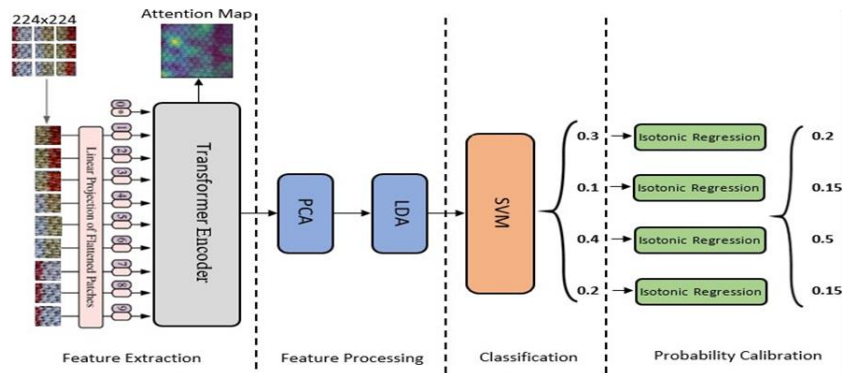
\includegraphics[width=\linewidth]{images/Paper3Model.png}
    \end{minipage}
    \caption[Model architecture - Chitra G M et al.~\cite{chitra2023fabric}]{Model architecture used for fabric composition identification in Chitra G M et al.~\cite{chitra2023fabric}}
\end{figure}

The model achieves an average F1-score of 0.87, along with a mean squared error (MSE) of 0.20 and a log-loss of 0.44. These results show that the pipeline is capable of reliably identifying both pure and mixed fabric types. Additionally, the use of SHAP (SHapley Additive exPlanations) values provides interpretability to the model by highlighting which parts of the image influenced the classification decision. This is especially useful in understanding how the model distinguishes between blended materials.

Overall, this work demonstrates the potential of Vision Transformers in fabric composition analysis. Its hybrid approach—combining ViTs with traditional dimensionality reduction and machine learning classifiers—offers a practical solution for real-world applications, including quality assurance, textile recycling, and online garment classification.
